% !TEX root = ./docs.tex

Bei der Implementierung wird Java 11 eingesetzt.
\subsection{Server}
Einstiegspunkt des Servers ist der Serverbootstrapper. Dieser erstellt einen neuen Thread mit einem neuen Server. 
\lstinputlisting[linerange={7-11}, firstnumber=7]{../src/main/java/vs/chat/server/ServerBootstrapper.java}
Der Server erstellt die Listener, die die zu empfangenen Pakete behandeln werden. Anschließend werden die Filter erstellt, die bestimmen, ob ein Paket gehandelt oder ignoriert werden soll (z.\,B. bei rekursiven Broadcasts).
\lstinputlisting[linerange={64-80}, firstnumber=64]{../src/main/java/vs/chat/server/Server.java}

Die Listener und die Filter werden in einen ServerContext gepackt, der mit allen Threads geteilt wird.
\clearpage

\begin{figure}[h]
    \centering
    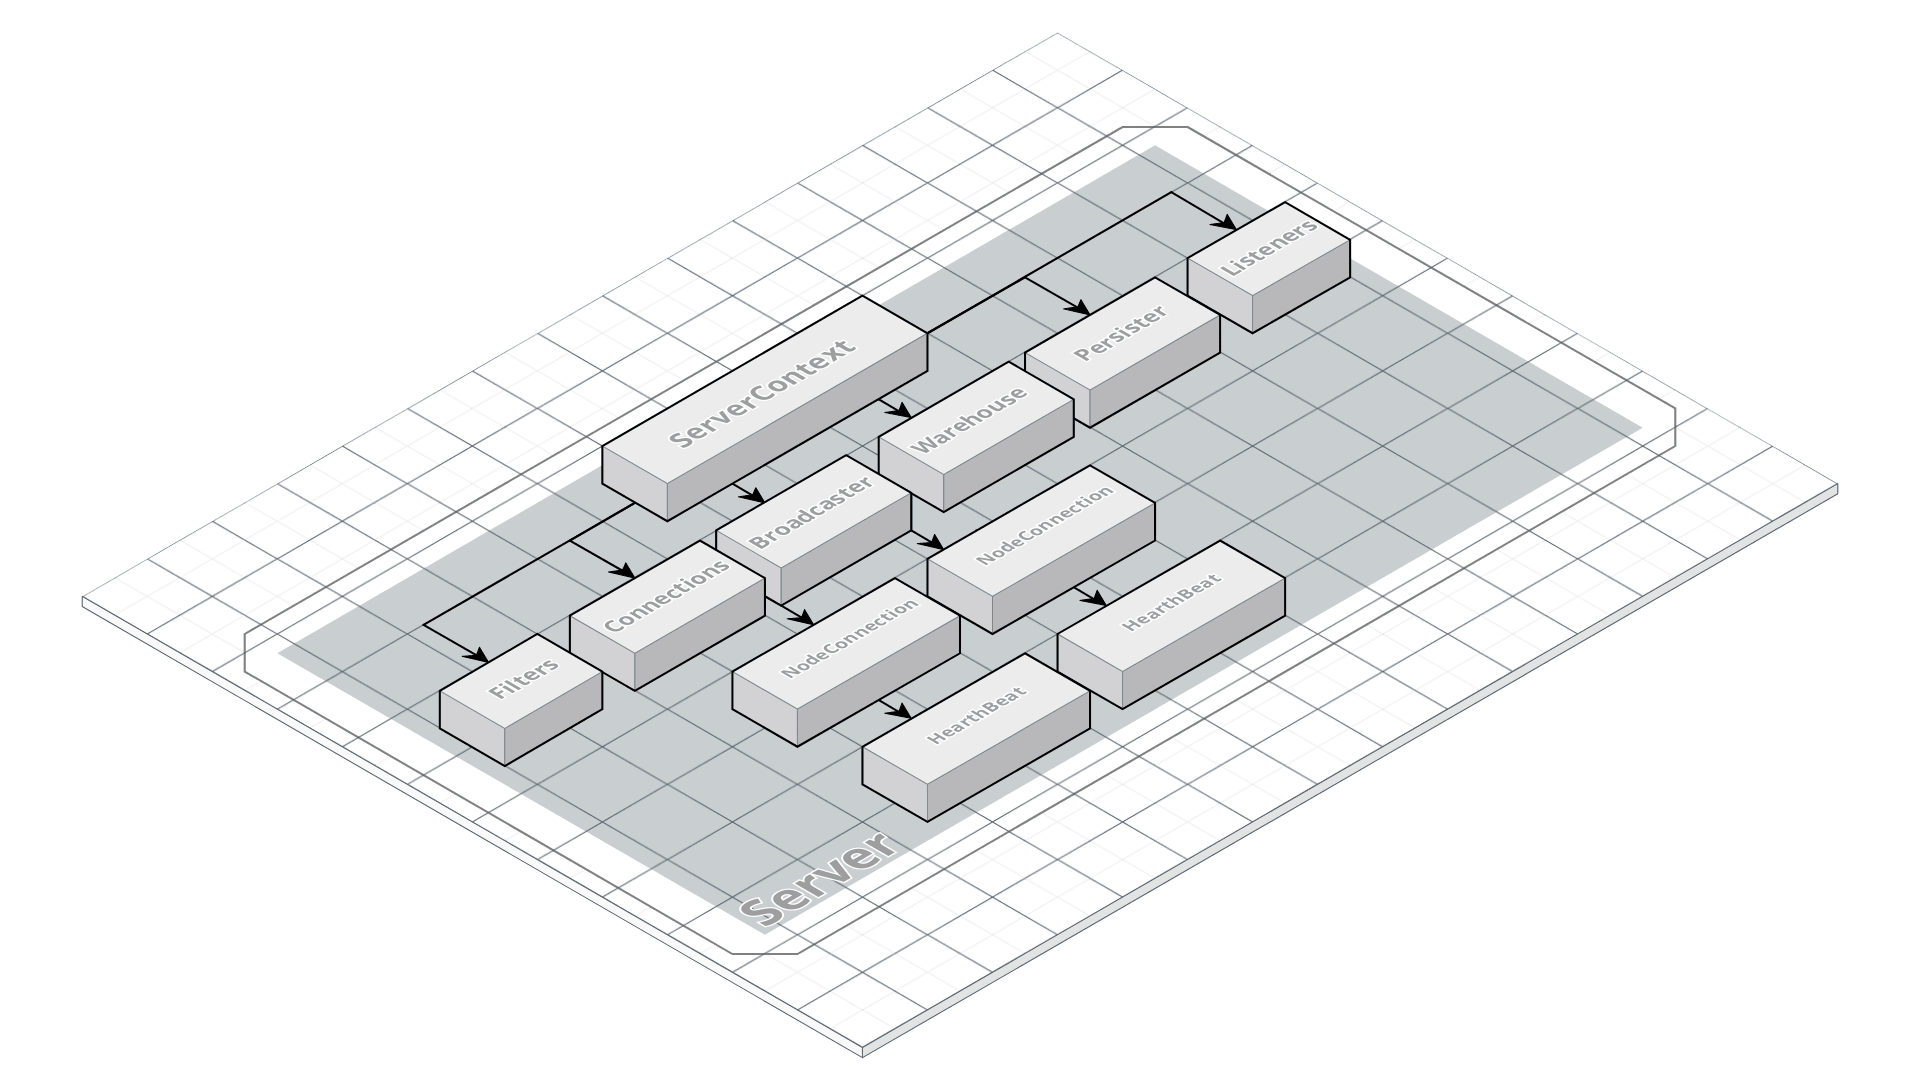
\includegraphics[width=\textwidth]{VS-Server-Context.png}
    
    \caption{Server-Context Aufbau}
\end{figure}


Sobald der ServerContext instanziiert wird, wird das Warehouse geladen. 
Zunächst wird versucht die Safe-Datei zu laden. Scheitert das Laden, wird das Warehouse leer instanziiert.

\lstinputlisting[linerange={53-64}, firstnumber=53]{../src/main/java/vs/chat/server/warehouse/Warehouse.java}


Das Warehouse hält sämtliche Daten, die persistiert werden müssen (z.\,B. Messages, Chats, Users). Der ServerContext erstellt außerdem den Persister. Der Persister ist ein Thread, der in regelmäßigen Abständen das Warehouse speichert.
\lstinputlisting[linerange={17-31}, firstnumber=17]{../src/main/java/vs/chat/server/persistence/Persister.java}
\lstinputlisting[linerange={66-75}, firstnumber=66]{../src/main/java/vs/chat/server/warehouse/Warehouse.java}
Alle Entitäten und Pakete haben eine UUID (Universally Unique Identifier) um diese zu unterscheiden. Verweise auf andere Entitäten (z.\,B. ein Chat hat mehrere Nutzer) werden ähnlich zu Fremdschlüsseln in relationalen Datenbanken umgesetzt. Die Entität speichert nur die UUID der Verknüpfung und nicht direkt die Information. Dies erlaubt eine feinere Synchronisation und reduziert mögliche Konfliktsituationen zwischen verschiedenen Nodes. Eingesetzt werden UUIDv4, die pseudozufällig erstellt werden. Dadurch sind zwar theoretisch Konflikte möglich, jedoch in Praxis sehr unwahrscheinlich.

Außerdem wird der Broadcaster erstellt, der die Verbindungen zu anderen Nodes hält und empfangene Nachrichten an diese verteilt.

\lstinputlisting[linerange={14-27}, firstnumber=14]{../src/main/java/vs/chat/server/node/NodeBroadcaster.java}


Weitere Variablen sind \textit{isCloseRequested}, die die 'endlos' Schleifen aller Threads steuert und \textit{connections}, welche alle Verbindungen zu Clients, die direkt zu dieser Node verbunden sind, hält.

Der Nodebroadcaster erstellt bei Instanziierung je Node einen eigenen Thread, der sich um das Senden und das neu Verbinden kümmert.
Nachrichten, die an eine Node gesendet werden sollen werden sollen werden vom Broadcaster in die Queue geschrieben und die NodeConnection wird durch einen Semaphor aufgeweckt. 
Die NodeConnection versucht eine Nachricht zu senden. Scheitert das Senden wird von einer Verbindungstrennung ausgegangen und die Verbindung wird neu aufgebaut.

\lstinputlisting[linerange={37-50}, firstnumber=37]{../src/main/java/vs/chat/server/node/NodeConnection.java}
Zusätzlich besitzt die NodeConnection jeweils einen HeartBeat-Thread. Dieser Thread sendet regelmäßig einen Ping, um zu testen, ob die Verbindung noch steht.
\lstinputlisting[linerange={16-25}, firstnumber=16]{../src/main/java/vs/chat/server/node/NodeHeartBeatThread.java}

Nachdem nun alle Initialisierungsvorgänge abgeschlossen sind, kann der ServerSocket erstellt und Clients akzeptiert werden.
Der Hauptserver-Thread ist dabei nur zuständig neue Verbindungen entgegenzunehmen. Für jede Verbindung wird ein ConnectionHandler-Thread erstellt, der sämtliche Nachrichten des Clients verarbeitet.
\lstinputlisting[linerange={41-60}, firstnumber=41]{../src/main/java/vs/chat/server/Server.java}

Nachrichten zwischen Servern und Clients werden als Pakete ausgetauscht. Der Handler versucht dabei ein Paket vom Client zu lesen. Die Filter prüfen nun, ob das Paket gehandelt werden darf (und nach dem Verarbeiten dessen werden diese aktualisiert).
\lstinputlisting[linerange={47-53}, firstnumber=47]{../src/main/java/vs/chat/server/ConnectionHandler.java}
Anschließend werden die passenden Listener gesucht und diese mit dem Paket aufgerufen.
\lstinputlisting[linerange={63-89}, firstnumber=63]{../src/main/java/vs/chat/server/ConnectionHandler.java}



Filter:
\begin{itemize}
    \item PacketIdFilter\\
        Der PacketId-Filter testet, ob ein Paket mit der Id bereits gesehen wurde. Nur wenn die Id neu ist darf das Packet gehandelt werden, um rekursive Broadcasts zu vermeiden. Bereits gesehene Pakete werden im Warehouse mitgespeichert. Im seltenen Fall, dass die Node genau zwischen den Listenern und dem Aktualisieren der Filter abstürzt kann es vorkommen, dass die gespeicherten Paket-ids nicht konsistent zum Nutzdatenbestand sind. Hier könnte ein Transaktionsprotokoll implementiert werden. Da aber die Wahrscheinlichkeit dieses Fehlers äußerst gering ist wird hier darauf verzichtet.
        \lstinputlisting[linerange={9-17}, firstnumber=9]{../src/main/java/vs/chat/server/filter/PacketIdFilter.java}
\end{itemize}



Listener:
\begin{itemize}
    \item BaseEntityBroadcastListener\\
        Der Listener behandelt BaseEntityBroadcastPackete, die ausgestrahlt werden, sobald ein neuer Nutzer, ein neuer Chat oder eine neue Nachricht erstellt wird. Die empfangene Entität wird in das Warehouse aufgenommen und weiter gesendet, falls es dieser Node neu war.
        \lstinputlisting[linerange={22-28}, firstnumber=22]{../src/main/java/vs/chat/server/listener/BaseEntityBroadcastListener.java}
        Nachdem ein Chat erstellt wurde müssen die Clients, die an diesem Chat teilnehmen informiert werden. Da jede Node nur die direkt zu ihr verbundenen Clients kennt, muss jede Node prüfen ob sie einen teilnehmenden Client kennt und diesen informieren. Ähnliches gilt für neue Nutzer.
        \lstinputlisting[linerange={33-50}, firstnumber=33]{../src/main/java/vs/chat/server/listener/BaseEntityBroadcastListener.java}
    \item CreateChatListener\\
        Dieser Listener erstellt Chats anhand von einem CreateChatPacket. Sofern das Paket von einem Nutzer kommt, wird ein neuer Chat mit allen Teilnehmern und dem Absender erstellt und weiter verteilt.
        \lstinputlisting[linerange={23-41}, firstnumber=23]{../src/main/java/vs/chat/server/listener/CreateChatListener.java}
    \item GetMessagesListener\\
        Mithilfe eines GetMessagePackets können alle Nachrichten abgefragt werden, die in einem Chat gesendet wurden.
        \lstinputlisting[linerange={20-32}, firstnumber=20]{../src/main/java/vs/chat/server/listener/GetMessagesListener.java}
    \item KeyExchangeListener\\
        Dieser Listener leitet KeyExchangePackete von einem Client an andere Clients weiter (gegebenenfalls über andere Nodes).
        \lstinputlisting[linerange={15-27}, firstnumber=15]{../src/main/java/vs/chat/server/listener/KeyExchangeListener.java}
    \item LoginListener\\
        Der LoginListener kümmert sich um die Authentifizierung eines Clients. Er prüft, ob ein Nutzer besteht und falls ja wird das Passwort geprüft.
        Außerdem wird die Information der Connection gesetzt, zu welchem Client sie verbunden ist, um ein gezieltes Senden zu ermöglichen (wie z.\,B. beim KeyExchange oder bei Messages).
        \lstinputlisting[linerange={25-34}, firstnumber=25]{../src/main/java/vs/chat/server/listener/LoginListener.java}
        Existiert noch kein Nutzer, wird ein passender Nutzer erstellt.
        \lstinputlisting[linerange={37-56}, firstnumber=37]{../src/main/java/vs/chat/server/listener/LoginListener.java}
        Anschließend wird der Client auf den neuesten Stand gebracht indem ein LoginSyncPacket an den Client gesendet wird. Dieses enthält die User-Id des aktuellen Nutzers, die anderen registrierten Nutzer und alle Chats, an dem der Client teilnimmt.
        \lstinputlisting[linerange={59-65}, firstnumber=59]{../src/main/java/vs/chat/server/listener/LoginListener.java}
    \item MessageListener\\
        Messages, die vom Client an einen Chat gesendet werden, werden von diesem Listener bearbeitet. Der Listener kümmert sich dabei auch um die Verteilung der Nachrichten an alle anderen Chatteilnehmer.
        \lstinputlisting[linerange={24-44}, firstnumber=24]{../src/main/java/vs/chat/server/listener/MessageListener.java}
    \item NodeSyncListener\\
        Wie in Fehlerbehandlung beschrieben müssen Nodes auf dem neuesten Stand gezogen werden, falls diese ausgefallen waren. Bei einem Reconnect wird ein NodeSyncPacket mit den aktuellen Informationen an die neu startende Node gesendet. Dieser Listener verarbeitet diese Pakete indem er prüft ob eine Änderung vorliegt und wenn ja diese übernimmt und broadcastet. 
        \lstinputlisting[linerange={16-34}, firstnumber=16]{../src/main/java/vs/chat/server/listener/NodeSyncListener.java}
        Theoretisch kann es sein, dass ein Nutzer sich anmeldet bevor die Node ihre Synchronisation abgeschlossen hat. Dieser Fehlerfall wird aber nicht weiter behandelt, da die Synchronisationszeit und die Ausfallwahrscheinlichkeit einer Node als zu gering eingestuft wird.
\end{itemize}

\subsection{Client}
API-Funktionen
\begin{itemize}
    \item Funktion - login\\
    Bei der Funktion login werden der Benutzername und das Passwort des Benutzers entgegengenommen. Diese werden als neues LoginPacket an den Server geschickt. Dort wird unter anderem überprüft, ob es sich um einen neuen Nutzer handelt (es wird ein Neuer angelegt) oder es ein bereits existierender Nutzer ist (Passwort wird überprüft). An dieser Stelle wartet der Client auf ein LoginSyncPacket (Login war erfolgreich). Danach werden die Attribute (userId, chats, contacts) abgespeichert. Für die Verschlüsselung wird auch noch die Keyfile geladen, in der die Schlüssel der eigenen Chats gespeichert sind. Sollte es noch keine Keyfile geben, wird eine neue erzeugt. Diese Datei ist ähnlich wie die Warehouse-Datei aufgebaut (hier wird über die Chat-Id, die Schlüssel geladen). Abschließend wird aus den beiden festgeschriebenen, öffentliche Primzahlen noch ein Schlüssel generiert, der später für den Diffie-Hellman-Key-Exchange notwendig ist.
    \lstinputlisting[linerange={126-156}, firstnumber=126]{../src/main/java/vs/chat/client/ClientApiImpl.java}
    \item Funktion - generatePrivateKey\\
    Mit dieser Funktion wird ein 128 Schlüssel aus den beiden öffentlichen Primzahlen n und g generiert. Der Schlüssel wird für die Verschlüsselung verwendet.
    \lstinputlisting[linerange={166-174}, firstnumber=166]{../src/main/java/vs/chat/client/ClientApiImpl.java}
    \item Funktion - exchangeKeys\\
    Um den Diffie-Hellman-Key-Exchange zu starten muss die \textit{exchangeKeys} Methode vom Client aufgerufen werden.
    Dabei erstellt die Methode das erste KeyExchangePacket, welches mit den erforderlichen Informationen
    ausgestattet wird. Nachdem das Paket gesendet wurde, haben die Teilnehmer zehn Sekunden Zeit, um den Schlüsseltausch durchzuführen.
    Wenn dies innerhalb der angegebenen Zeit nicht geschieht, wird von einem Fehler ausgegangen und die Error-Handling-Methode \textit{onTimeout} aufgerufen.
    \lstinputlisting[linerange={202-223}, firstnumber=202]{../src/main/java/vs/chat/client/ClientApiImpl.java}
    \item Funktion - createChat\\
    Für einen neuen Chat werden zwei Parameter benötigt: Der Name des Chats und eine Liste mit Usern. Um einen neuen Chat zu
    erstellen, wird ein CreateChatPacket mit dem Chatnamen und einem Array der User-Ids an den Server geschickt.
    \lstinputlisting[linerange={225-232}, firstnumber=225]{../src/main/java/vs/chat/client/ClientApiImpl.java}
    \item Funktion - sendMessage\\
    Hier wird die eigentliche Nachricht und eine Chat-Id entgegengenommen. Diese werden dann in ein MessagePacket an
    den Server geschickt.
    \lstinputlisting[linerange={234-240}, firstnumber=234]{../src/main/java/vs/chat/client/ClientApiImpl.java}
    \item Funktion - Verschlüsselung (encryptAES, decyptAES, setKey) \\
    Für die symmetrische Verschlüsselung der Nachrichten wird der AES-Algorithmus benutzt. Hierfür wird vor jedem Senden
    die Methode \textit{encryptAES} und nach jeder empfangener Nachricht \textit{decryptAES} aufgerufen.\\
    Für die Verschlüsselung wird zunächst der Schlüssel in das richtige Format (SecretKeySpec), durch die Funktion
    \textit{setKey} gebracht. Anschließend wird eine Instanz der Klasse Cipher erzeugt und mit dem Verschlüsselungsmodus und
    dem Key initialisiert. Abschließend wird der eigentlich Text verschlüsselt und in einem String zurückgegeben. \\
    Die Entschlüsselung ist fast identisch zur Verschlüsselung. Hier wird die Instanz in dem Entschlüsselungsmodus
    initialisiert.
    \lstinputlisting[linerange={235-255}, firstnumber=235]{../src/main/java/vs/chat/client/ClientApiImpl.java}
    \item Funktion - Keyfile (addKey, loadKey, deleteKey) \
    addKey\\
    Mit diesen Funktionen wird auf die Keyfile des Benutzers zugegriffen. Die Keyfile besteht aus PrivateKeyEntitys.
    Der Schlüssel ist die chatId.
    Wird ein neuer Key gespeichert, wird eine neue PrivateKeyEntity mit der chatId und dem Schlüssel in der keyfile
    abgespeichert.
    
    loadKey\\
    Müssen Nachrichten angezeigt werden, muss der Schlüssel aus der Datei für die chatId ausgelesen werden.
    
    deleteKey \\
    Sollte ein Chat irgendwann gelöscht werden, kann der die PrivateKeyEntity über die chatID entfernt werden. 
    
    \lstinputlisting[linerange={257-301}, firstnumber=257]{../src/main/java/vs/chat/client/ClientApiImpl.java}
    \item Funktion - exit \\
    Bei dieser Methode wird ein LogoutPacket an den Server geschickt. Der User wird hier noch nicht ausgeloggt!
    \lstinputlisting[linerange={312-316}, firstnumber=312]{../src/main/java/vs/chat/client/ClientApiImpl.java}
    \item PacketListener-Thread \\
    Dieser Thread läuft die gesamte Zeit im Hintergrund und nimmt alle (außer LoginSynPacket) Packete, die vom Server
    an den Client geschickt werden, auf und verarbeitet sie.
    Zuerst wird überprüft, ob es sich um ein BaseEntityBroadcastPacket handelt. Anschließend gibt es verschiedene Möglichkeiten: \\
    \begin{enumerate}
        \item Es wurde ein Chat erstellt, in dem der User enthalten ist. Hier wird der Key in der Keyfile abgespeichert
        und der Chat zu den Chats des Users hinzugefügt.
        \item Es wurde eine Nachricht an den User geschrieben. Hier wird der Schlüssel aus der Keyfile geladen und die
        Nachricht damit entschlüsselt.
        \item Es hat sich ein neuer User angemeldet. Dieser User muss den Usern des Clients hinzugefügt werden, damit auch
        Chats mit diesem erstellt werden können. (Diffie Hellman funktioniert nur, wenn alle Nutzer online sind.)
    \end{enumerate}
    \lstinputlisting[linerange={326-356}, firstnumber=326]{../src/main/java/vs/chat/client/ClientApiImpl.java}
    Handelt es sich um ein KeyExchangePacket, wird überprüft, ob der Schlüsseltausch schon fertig ist,
    falls ja erstellt der Initiator des Schlüsseltauschs den Chat, falls nicht werden die nächsten
    Teilschlüssel berechnet und weitergeschickt.\\
    \lstinputlisting[linerange={358-403}, firstnumber=358]{../src/main/java/vs/chat/client/ClientApiImpl.java}
    Wird ein GetMessagesResponsePacket erhalten, wurde an den Server zuvor die Anfrage gestellt, dass die Chat Historie
    geladen werden soll. Dieses Packet enthält alle Nachrichten, die in dem geladenen Chat bereits geschrieben wurden.
    Dafür wird zunächst der passende Schlüssel aus der Keyfile geladen und danach alle Nachrichten entschlüsselt.
    Diese Nachrichten können dann im Chat angezeigt werden.\\
    \lstinputlisting[linerange={405-419}, firstnumber=405]{../src/main/java/vs/chat/client/ClientApiImpl.java}
    Abschließend wird geprüft, ob es ein LogoutSuccessPacket ist. Dieses Paket wird vom Server geschickt, wenn der
    User die exit Methode aufgerufen hat und erfolgreich vom Server ausgeloggt wurde. Anschließend wird der Client
    heruntergefahren.\\
    \lstinputlisting[linerange={430-438}, firstnumber=430]{../src/main/java/vs/chat/client/ClientApiImpl.java}
Verwendung von Emojis: \\\\
	Wie bereits in der Doku erwähnt nutzen wir für die Darstellung von Emojis Unicode.
	\lstinputlisting[linerange={621-631}, firstnumber = 621]{../src/main/java/vs/chat/client/UI/ClientGUI.java}
	Die im String Array unicodeemoji erhaltenen Unicode Zeichen werden jeweils in einem JLabel hinzugefügt und auf ein Panel gesetzt. Jedes JLabel bekommt den selben Mouselistener zugewiesen, der als Übergabeparameter das entsprechende Unicodezeichen erhält. Im EmojiMouselistener wird mit der Funktion append() die JTextArea um das jeweils übergebene Unicodezeichen erweitert.
	\lstinputlisting[linerange={89-109}, firstnumber = 89]{../src/main/java/vs/chat/client/UI/ClientGUI.java}
	Durch das Erweitern oder Ändern des unicodeemoji Arrays können die Emoticons getauscht oder beliebig erweitert werden. Weiter Anpassungen sind nicht nötig.
\end{itemize}


